\documentclass[review]{elsarticle}

\usepackage{lineno,hyperref}
\modulolinenumbers[5]
\usepackage[margin=2cm]{geometry}
\usepackage{amsmath}
\usepackage{subcaption}
\usepackage{graphicx}
\usepackage[justification=centering]{caption}
\usepackage{tikz}
\journal{Ecological Informatics}

%%
%% Guide for authors : https://www.elsevier.com/journals/ecological-informatics/1574-9541/guide-for-authors
%%
%%
%% Editor Latex instructions : https://www.elsevier.com/authors/author-schemas/latex-instructions
%%



%%%%%%%%%%%%%%%%%%%%%%%
%% Elsevier bibliography styles
%%%%%%%%%%%%%%%%%%%%%%%
%% To change the style, put a % in front of the second line of the current style and
%% remove the % from the second line of the style you would like to use.
%%%%%%%%%%%%%%%%%%%%%%%

%% Numbered
%\bibliographystyle{model1-num-names}

%% Numbered without titles
%\bibliographystyle{model1a-num-names}

%% Harvard
%\bibliographystyle{model2-names.bst}\biboptions{authoryear}

%% Vancouver numbered
%\usepackage{numcompress}\bibliographystyle{model3-num-names}

%% Vancouver name/year
%\usepackage{numcompress}\bibliographystyle{model4-names}\biboptions{authoryear}

%% APA style
%\bibliographystyle{model5-names}\biboptions{authoryear}

%% AMA style
%\usepackage{numcompress}\bibliographystyle{model6-num-names}

%% `Elsevier LaTeX' style
\bibliographystyle{elsarticle-num}
%%%%%%%%%%%%%%%%%%%%%%%

\begin{document}

\begin{frontmatter}

  \title{Automated Morphometrics using Deep Neural Networks : Case Study on a Beneficial Insect Species}

%\tnotetext[mytitlenote]{Fully documented templates are available in the elsarticle package on \href{http://www.ctan.org/tex-archive/macros/latex/contrib/elsarticle}{CTAN}.}



%% Group authors per affiliation:
\author[labri,itdlu]{Le Van Linh\corref{cor1}}
\ead{van-linh.le@labri.fr}
\author[labri]{Zemmari Akka}
\author[igepp]{Marie Alexia (?)}
\author[labri]{Beurton-Aimar Marie\fnref{ba}}
\author[igepp]{Parisey Nicolas\fnref{ba}}

\fntext[ba]{both authors contributed equally to this work.}
\cortext[cor1]{Corresponding author} 

%% %% or include affiliations in footnotes:
\address[igepp]{UMR 1349 IGEPP, BP 35327, 35653 Le Rheu, France}
%% \ead[url]{www.elsevier.com}

\address[labri]{University of Bordeaux, 351, cours de la Libération, 33405 Talence}
\address[itdlu]{Dalat University, Dalat, Lamdong, Vietnam}
%% \cortext[mycorrespondingauthor]{Corresponding author}
%% \ead{support@elsevier.com}

%% \address[mymainaddress]{1600 John F Kennedy Boulevard, Philadelphia}
%% \address[mysecondaryaddress]{360 Park Avenue South, New York}

\begin{abstract}
\textit{Aims:} \ldots \textit{Methods:} \ldots \textit{Conclusions:} \ldots
Landmark is one of the important concepts in morphometry analysis. Finding landmarks is not only used to measure the shape of the object but also applied to analyze the inter-organisms variations. Currently, the landmarks are mostly determined manually by the biologist.
In this work, we propose a method to automatic predict the landmarks on biological images: Deep Learning, more specific is Convolutional Neural Network (CNN). We proposed a CNN architecture which was built from the ``elementary blocks". Each block is made up of some popular layers of CNN.
The network then trained and tested on a dataset includes five parts of beetle (head, elytra, pronotum, left and right mandibles).
These works have also introduced another procedure to augment the dataset which can see a little bit small in our case.
In the experiments, we apply two strategies to evaluate the network and to improve the obtained results: training from scratch and applying a fine-tuning step.
The predicted landmarks from the network have been compared with the manual landmarks which provided by the biologists. The obtained results have proved that the predicted landmarks are considered to be statistically good enough to replace the manual landmarks.
\end{abstract}

\begin{keyword}
Landmarks \sep morphometry \sep deep learning \sep CNN
\end{keyword}

\end{frontmatter}

\linenumbers

\section{Introduction}

In the context of ecosystem services, there is an interest in studying complex interactions between evolution of insect populations and environmental factors affecting their functions. In order to assess specifically pest-regulating services and in line with studies pointing to shape traducing function \cite{klingenberg_evolution_2010}, there are more and more research about beneficial insect morphometrics \cite{sasakawa_utility_2016,raymond_combination_2014}. 
 In such morphometric studies, it is common to analyze subject's shape independently of their poses and sizes \cite{kendall_diffusion_1977}. Since the late $20^{th}$ century \cite{bookstein_foundations_1982}, rooted in a strong statistical background, geometric morphometrics addresses the study of such biological shapes \cite{rohlf_applications_1998}. It is an effective set of methods with several specialised softwares readily available \cite{adams_geomorph:_2013,klingenberg_morphoj:_2011}. Classical geometric morphometrics uses a set of landmarks to describe shape, a landmark being a two-dimensional anatomically-relevant point. In order to investigate the possibility of automated morphometric geometrics on beneficial insects, we chose to focus on one of the most common and ubiquitous beneficial insect of north-western France, \textit{Poecilus cupreus} (Carabidae). It is considered a polyphagous predator \cite{larochelle_1990} beneficial to agriculture, being able to consume a large variety of agricultural pests including weed seeds, slugs and aphids \cite{kromp_carabid_1999}. As a Coleoptera, its morphological variability is usually measured on exoskeleton structures such as the head, pronotum and elytra \cite{eldred_does_2016}. \\
 
Of course, the first step in any morphometric geometrics study is the digital imaging of the biological specimens, usually with controlled illumination and contrasting background. As such, morphometric landmark detection and positioning can be though as a particular problem of features detection and solved using robust digital image processing \cite{gonzalez_digital_2006}. In the recent years, the term ``deep learning" emerged describing class of computational models composed of multiple processing layers learning representations of data with multiple levels of abstraction \cite{lecun2015deep}. Each layer extracts the representation of the input data from the previous layer and computes a new representation for the next layer. In the hierarchy of model, higher layers of representation enlarge aspects of the input that is important for the computational task (classification, regression, \ldots) and suppress irrelevant variations. As supervised learning algorithms, they use gradient descent optimization method to update the learnable parameters via backpropagation. Deep learning algorithms have proved to be very efficient in a wide variety of domains, notably image recognition and classification \cite{krizhevsky2012imagenet,ciregan2012multi,szegedy2015going}, speech recognition \cite{mikolov2011strategies, hinton2012deep, sainath2013deep}, question answering \cite{bordes2014question} and language translation \cite{sutskever2014sequence, jean2014using}.
Within deep learning, Convolutional Neural Networks (CNNs) are well known for their success in many computer vision tasks such as image classification \cite{krizhevsky2012imagenet,ciregan2012multi} and  objets recognition \cite{li2015convolutional,tompson2014joint}.
Recent success of this algorithm in human biometry \cite{cintas2016automatic} lead us to believe in its potential for insect morphometrics.  

\subsection{Related works}\label{rw}

Landmark or point of interest is a specific point that may contain the useful information. For example, the tip of the nose or the corners of the mouth are landmarks on human face. In image processing, we can consider two kinds of cases: the object of interest can or not be segmented. Setting landmarks can not be achieved in the same way depending on which situation we are. When segmentation can be applied, Lowe et al. \cite{lowe2004distinctive} have proposed SIFT method to find the corresponding keypoints between two images. Palaniswamy et al. \cite{palaniswamy2010automatic} have proposed a method based on probabilistic Hough Transform to automatically locate the landmarks in digital images of Drosophila wings. In our work \cite{le2017maelab}, we have proposed a method which have been extended from Palaniswamy's method, to determine landmarks on mandibles of beetles. The mandibles of beetle have the simple shape and easy to segment. We have obtained good enough results about determining the landmarks automatically on mandibles. Unfortunately, this method can not be applied to other parts of beetles than the pronotum seems is segmentation has too many noises.

In recent years, deep learning is known as a solution in computer vision. Using convolutional network to determine the landmarks on 2D images has achieved better results and it seems that good solutions for the images that can not segment. Yi Sun et al. \cite{sun2013deep} have proposed cascaded convolutional neural networks to predict the facial points of interest on the human face.
Zhanpeng Zhang et al. \cite{zhang2014facial} proposed a \textit{Tasks-Constrained Deep Convolutional Network} to optimize facial landmarks detection. The model determines the facial landmarks with a set of related tasks such as head pose estimation, gender classification, age estimation, face recognition, or facial attribute inference. In biology field, Cintas et al. \cite{cintas2016automatic} has introduced a network to predict the landmarks on human ears. After training, the network has the ability to predict 45 landmarks on human ears. In this way, we have applied CNN computing to work with pronotum landmarks.

\subsection{Contributions}

We present an approach to predict morphometric landmarks based on standardized digital pictures of a coleoptera anatomical parts. For each anatomical parts, we train a convolutional neural network and statisticaly assess the suitability of the predicted landmarks to replace manual landmarks in further geometric morphometric studies.

\section{Material and Methods}

In the context of this section, we first present the dataset that we have used in this study, as well as the strategies to pre-process the data. Then, we show the network architecture model that we have designed to predict the landmarks in the beetle's images.

\subsection{Dataset and preprocessing}
In order to provide the experiment data, we have selected the Brittany lands (North-West of France) to collect the samples. After collecting in three months, a collection of $293$ beetles has been established ($147$ males and $146$ females/ $155$ organic and $138$ conventional) (Figure \ref{imgbeetle}). As usual, images of beetles have been chosen to be studied instead of using real objects for pratical reasons. The pictures of each body parts were captured under a trinocular magnifier at $\approx 300$ pixels/mm for elytra, $\approx 600$ pixels/mm for pronotum and head, $1500$ pixels/mm for mandibles. One can note that the head, pronotum, and elytra parts have been captured before dissection. The Lleft and right mandibles have been separated from the beetle's body before taking the photos. All the images have been taken with the same camera under same conditions to release in the RGB color mode with the size of $3264 \times 2448$.

\begin{figure}[h!]
	\centering
	\begin{tikzpicture}
		\node (img1) {\includegraphics[width=0.60\textwidth]{images/beetle2}};
		\draw[thick,<->] (-3.2,-2.5) -- (4.7,-2.5);
		\node at (1, -2.7) {\footnotesize{12 mm}};	
	\end{tikzpicture}
	\caption{An illustration of the beetle.}
	\label{imgbeetle}
\end{figure}

In the next step, morphological landmarks were first set manually on the dorsal views of each body part of the beetles (head, pronotum, elytra, right and left mandibles). The morphology of each body part was processed and analyzed separately in order to limit variation resulting from their relative positions due to articulation. Landmarks were chosen according to the ease and the precision of their location on each specimen (Figure \ref{figdatasamples}). Replicability analyses were performed to confirm the accuracy of landmarks positioning. They were positioned on each picture with TPSDig2 software (version 2.17) (Rohlf, 2013a). In some individuals, mandibles could not be processed because they were lacking or broken. For each specific part, a set of number of landmarks has been provided, for example, \textit{$8$ landmarks for pronotum, $10$ landmarks for head, $11$ landmarks for elytra, $16$ and $18$ landmarks for left and right mandibles, respectively} (Figure \ref{figdatasamples}). In the context of this study, these manual landmarks have been used as ground truth to evaluate the output of our method.

\begin{figure}[h!]
    \centering
    \subcaptionbox{. Pronotum.}{\includegraphics[width=0.19\textwidth]{./images/Prono_010}}~~
\subcaptionbox{. Head.}{\includegraphics[width=0.19\textwidth]{./images/Tete_009}}~~
\subcaptionbox{. Elytra.}{\includegraphics[width=0.19\textwidth]{./images/Elytre119}}~~
\subcaptionbox{. Left mandible.}{\includegraphics[width=0.19\textwidth]{./images/Mg_021}}~~
\subcaptionbox{. Right mandible.}{\includegraphics[width=0.19\textwidth]{./images/Md_015}}~\\
	\subcaptionbox{. Pronotum.}{\includegraphics[width=0.19\textwidth]{./images/pronotum_mlm}}~~
\subcaptionbox{. Head.}{\includegraphics[width=0.19\textwidth]{./images/tete_mlm}}~~
\subcaptionbox{. Elytra.}{\includegraphics[width=0.19\textwidth]{./images/elytre_mlm}}~~
\subcaptionbox{. Left mandible.}{\includegraphics[width=0.19\textwidth]{./images/lmandible_mlm}}~~
\subcaptionbox{. Right mandible.}{\includegraphics[width=0.19\textwidth]{./images/rmandible_mlm}}~\\
    \caption{The sample images in our dataset (top row) and manual landmarks on each part defined by biologists (bottom row).}
    \label{figdatasamples}
\end{figure}

The success stories \cite{} have proved that CNN models have been trained on a large dataset with an enormous number of data samples before using it to perform on testing data. Training the model with a big dataset can help the model able to learn more different cases and to improve the learning ability of the network. Unfortunately, providing a large dataset is too costly in several domains, e.g., in biology, medical. A solution to deal with this problem is to create the misshapen data from real data and to add them to the dataset. In our case, we have only 293 images for each part of the beetles. This number is large from the point of view of manual operations, but it is not enough to apply deep learning methods. So, we have augmented the number of images in each set of images.

Most often in deep learning applications, dataset augmentation uses operations such as translation, rotation, or scaling, which are well-known efficient to generate the new version of existing images \cite{}. However, these operations can be invariant in some cases \cite{}. We have done some tests by moving the object in the picture. In each time, we have quickly gone to the over-fitting in the training step (more detail in Section X). Consequently, we have preferred different ways to produce misshapen images by operating on the image's color channels. We have proposed two strategies to augment the number of images in our dataset.

The first strategy was applied to change the value of each channel in the original image. According to this, a constant have been added to a channel of RGB image for each time. For example, if we add a constant $c = 10$ to the red channel from an original RGB image, we will obtain a new image with the values at red channel by greater than the red channel of original image a value of $10$. By this way, we can generate three new RGB images from a RGB image.

The second procedure was split the channels of RGB images to create three gray-scale images. This work seems promising because the network model on single-channel images. At the end, we have generated six versions from an image. In total, we have obtained $293 \times 7 = 2051$ images for each set of images. Figure \ref{figdataauge} illustrates the two strategies that we have described.

\begin{figure}[h!]
    \centering
    \subcaptionbox{. Add a constant to each channel.}{\includegraphics[width=0.49\textwidth]{./images/inc_channels}}~~
\subcaptionbox{. Split the channels of image.}{\includegraphics[width=0.49\textwidth]{./images/sp_channels}}
    \caption{The two strategies to augment the number of images in our dataset.}
    \label{figdataauge}
\end{figure}





In the content of this study, we work on pronotum part of beetle. The provided dataset contains 293 images, each image with 8 landmarks provided by biologists. The dataset was split into a training set with 260 images (training and validation) and a testing set of 33 images. During the training, the network learned the information through a pair of \textit{(image, landmarks)} in training set. At the testing phase, the image without landmarks was given to the trained network and the predicted landmarks will be given at the output. Fig. \ref{figpronotum} shows an example of pronotum image with its manual landmarks.

\begin{figure}[h!]
	\centerline{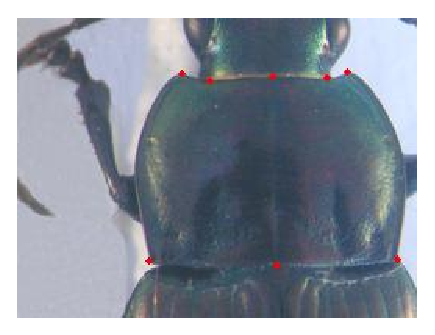
\includegraphics[scale=0.8]{images/pronotum}}
	\caption{An example of pronotum with manual landmarks}
	\label{figpronotum}
\end{figure}

In some succeed networks \cite{krizhevsky2012imagenet}\cite{sun2013deep}\cite{cintas2016automatic}, the maximum size of the inputs is not over 256 pixels. In our case, the resolution of the image is large, it becomes a difficulty for the network. During training and testing, the images are down-sampling to the new resolution of $256 \times 192$. Certainly, the landmark coordinates of the image are also scaled to suit their new resolution. 

The proposed network has a large number of learnable parameters. In addition, the size of the dataset is limited, this means that overfitting will occur during the training process. Therefore, we need to enlarge the size of the dataset. In image processing, we usually apply transform procedure (i.e rotate, translate) to generate a new image but in fact, when we compute the value of the pixels, it does not change while CNN computes the values of the pixels.Therefore, we have applied two other procedures to increase the number of images in the dataset. To address this problem, we have applied two procedures to enlarge the size of the dataset.

The first procedure was applied to change the value of each channel in the original image. According to this, a constant is added to a channel of RGB image and for each time, we just change the value of one of three channels. For example, from an original RGB image, if we add a constant $c = 10$ to the red channel, we will obtain a new image with the values at red channel by greater than the red channel of original image a value of 10. By this way, we can generate three new RGB images from a RGB image.

The second procedure is splitting the channels of RGB images. It means that we separate the channels of RGB into three gray-scale images. This work seems promising because the network works on single-channel images. At the end, we can generate six versions from an image, the total number of images used to train and validate is $260 \times 7 = 1820$ images (six versions and original image). The number of images that used for training and validation is splitted randomly by a ratio (training: $80\%$, validation: $20\%$) that has been set during the network setup.

In practical, when we work with CNN, convergence is usually faster if the average of each input variable over the training set is close to zero. Moreover, when the input is set closed with zero, it will be more suitable with the sigmoid activation function \cite{lecun2012efficient}. According to \cite{lecun2012efficient}, the brightness of the image is normalized to $[0,1]$, instead of $[0,255]$ and the coordinates of the landmarks are normalized to $[-1,1]$, instead of $[0,256]$ and $[0,192]$ before giving to the network.

\subsection{Network architecture and training}

\subsection{Measuring similarities between predicted and observed landmarks}

\section{Results}

\subsection{Automated landmarks prediction for different anatomical parts}

The dataset has been built by the biologists. It includes the images and manual landmarks. So, we can use the manual landmarks coordinates as ground truth to evaluate the coordinates of predicted landmarks. In the context of deep learning, landmark prediction can be seen as a regression problem. Therefore, the quality metric is used to evaluate the results. In particular, we use root mean square error (RMSE) to compute the accuracy of the implemented architecture. 
\begin{figure}[h!]
	\centerline{\includegraphics[scale=0.45]{images/loss_model_1}}
	\caption{Learning curves of the first model.}
	\label{figloss1}
\end{figure}~\\
\begin{figure}[h!]
	\centerline{\includegraphics[scale=0.45]{images/loss_v16}}
	\caption{Learning curves of the last model.}
	\label{figloss}
\end{figure}~\\[0.1cm]
Fig.\ref{figloss1} and \ref{figloss} show the training errors and the validation errors of a training time on the first and the third model, respectively. The blue curve presents RMSE on training set, the green curve presents the validation error. Clearly, the overfitting has appeared in the first model. In Fig.\ref{figloss1}, we can see that if the training is able to decrease with the number of epochs\footnote{An epoch is a single pass through the full training set.}, it is not the case of validation loss. At the opposite in the third model, we can see some different values for the two losses at the beginning but after several epochs, these values become more proximate and the overfitting problem has been solved.

Fig.\ref{figrsexample} shows the predicted landmarks on test images set by the thrid model. When we consider the distance between the predicted and manual landmarks, the accuracy on coordinates of predicted landmarks on Fig.\ref{figsub1} is $99\%$. The propotion on Fig.\ref{figsub2} is $80\%$.

\begin{figure}[h]
    \centering
    \begin{subfigure}[t]{0.25\textwidth}
        \centering
        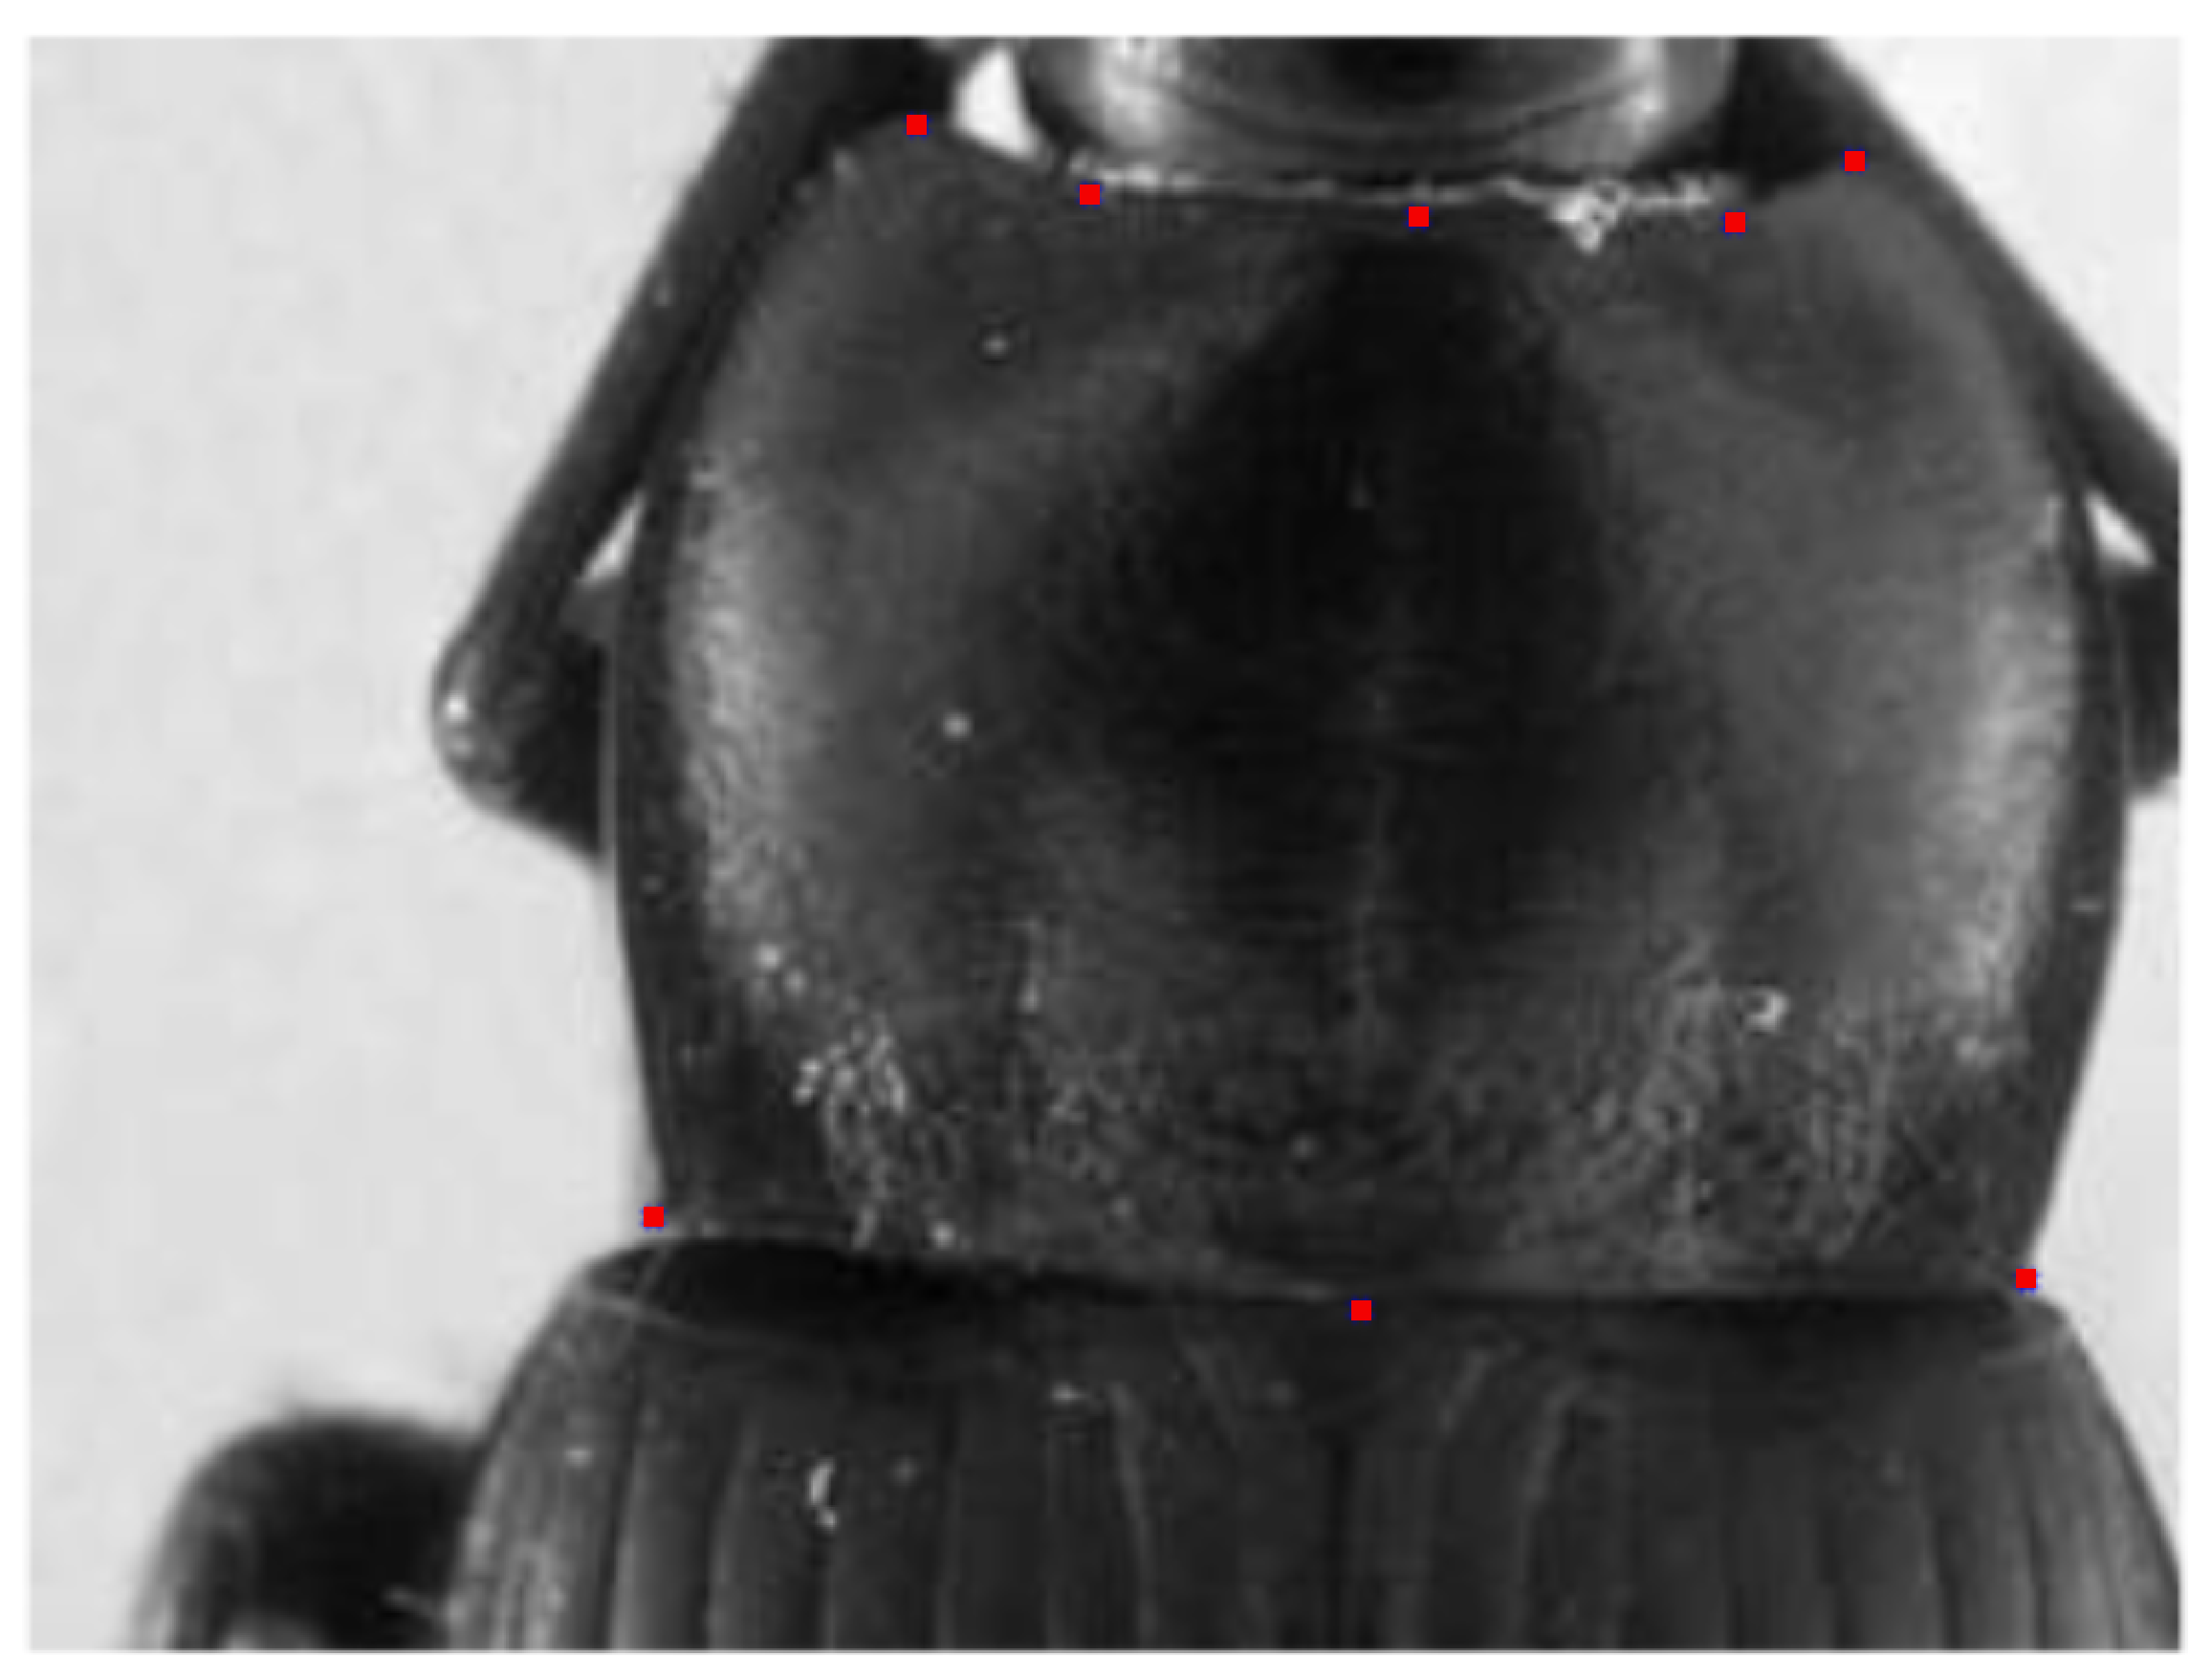
\includegraphics[height=1.2in]{images/plandmark}
        \caption{Image with well-predicted landmarks}
        \label{figsub1}
    \end{subfigure}%
    ~ 
    \begin{subfigure}[t]{0.25\textwidth}
        \centering
        \includegraphics[height=1.2in]{images/plandmark2}
        \caption{Image with inaccuracy landmarks}
        \label{figsub2}
    \end{subfigure}
    \caption{The predicted landmarks on an image in test set (red points)}\
    \label{figrsexample}
\end{figure}
Besides the losses of training, the distance from predicted landmarks to manual landmarks of the test images deserve attention also. Firstly, the distance between them is calculated. Then, the standard deviation \cite{bland1996statistics} is used to quantify the dispersion of a set of distances. Table.\ref{tab2} shows the average error distance given on each landmark.

\begin{table}[htbp]
\caption{The average distance per landmark}
\begin{center}
\begin{tabular}{|c|p{1.5cm}|}
\hline
\textbf{$\#$Landmark} & \textbf{Distance} \\ \hline
1 & 4.002  \\ \hline
2 & 4.4831 \\ \hline
3 & 4.2959 \\ \hline
4 & 4.3865 \\ \hline
5 & 4.2925 \\ \hline
6 & 5.3631 \\ \hline
7 & 4.636 \\ \hline
8 & 4.9363 \\ \hline
\end{tabular}
\label{tab2}
\end{center}
\end{table}

Fig.\ref{figchartlm1} shows the distribution of the distances on the first landmarks of all images. The accuracy based on the distance of each image can be separated into three spaces: the images have the distance less than average value ($4$ pixels): \textbf{56.66$\%$}; the images have the distance from average value to $10$ pixels: \textbf{40.27$\%$}; and the images have the distance greater than $10$ pixels: \textbf{3.07$\%$}. The network has enabled to detect the landmark on pronotum automatically. %If we consider the distance less than average value are good,

\begin{figure}[htbp]
	\centerline{\includegraphics[scale=0.3]{images/statistic}}
	\caption{The distribution of the distances on the first landmark. The blue line is the average value of all distances.}
	\label{figchartlm1}
\end{figure}
Fig.\ref{figchart} shows the proportion of acceptable landmarks. In our case, a predicted landmark is acceptable if the distance between it and corresponding manual landmarks is less than the average distance plus a value of standard deviation. Most of the landmarks have been detected with the accuracy greater than $70\%$. %However, we can see a vast difference between the correlation coefficient results and the proportions on each landmark.

\begin{figure}[htbp]
	\centerline{\includegraphics[scale=0.2]{images/chart}}
	\caption{The proportion of acceptable predicted landmarks}
	\label{figchart}
\end{figure}

At the test phase, the trained network is used to predict the landmarks on a set of test images. The program outputs the predicted-landmarks of the images as TPS files; in additional, it also fills and displays the predicted-landmarks on sixteenth firstly images of test data. With the outputs are TPS files, the user can use MAELab \cite{le2017maelab} framework\footnote{MAELab is a free software written in C++. It can be directly
and freely obtained by request at the authors.} to display the landmarks on the images.
\section{Conclusion and future works}
With beetle mandibles images, the object is easy to segment and we have succeeded to determine the landmarks automatically. In opposite, the pronotum images are difficult to segment. Methods which not suppose to be based on segmentation are necessary. In this paper, after testing several models, we have presented a convolutional neural network for automatic detection landmarks on the pronotum. It includes three times repeated structure which consists of a convolutional layer, a max pooling layer, and a dropout layer, followed by the connected layers. During the training phase, suitable techniques are used to prevent overfitting, a common issue of the neural networks. The network was trained several times in different selections of training data. After training with the manual landmarks given by the biologist, the network is able to predict the landmarks on the set of unseen images.

The results from the test set have been evaluated by calculating the distance between manual landmarks and corresponding predicted-landmarks. The average of distance errors on each landmark has been also considered. Using the convolutional network to predict the landmarks on biological images is promising good results in the case that the image can not be segmentation. The quality of prediction allows using automatic landmarking to replace manual landmarks in some aspects.  In our case, the training dataset is limited. As a result, the accuracy of the network is acceptable. However, when we expect more about the accuracy of predicted landmarks (coordinates of predicted landmarks), the result of this work is still needed to improve (for example using a larger training dataset). Therefore, future research in landmarking identification appears as an improved of the worth exploring.

\subsection{Evalution metrics for further predicted landmarks usage}

TODO \\

\section{Discussion}

TODO : a biological part, a computational part \\

\bibliography{includes/references}

\end{document}
